% ============================================================================
% Supplementary Material for main.tex (reSTITCHing), v10 (Overleaf build)
% ----------------------------------------------------------------------------
% Self-contained: compiles with pdflatex alone, with figures/ next to this file.
% ASCII only, no em-dashes. Sections S1..S9 are cited from the main text as
% "Supplementary Material Sn".
% Generated content (do not edit by hand): the NUMBERS and TABLES blocks
%   <- python -B phase2/frontier/make_numbers_set4.py
% figures/*.pdf <- python -B paper/make_v10_figures.py
% ============================================================================
\documentclass[11pt]{article}

\usepackage[margin=1in]{geometry}
\usepackage[T1]{fontenc}
\usepackage{amsmath}
\usepackage{newtxtext,newtxmath}
\usepackage[varqu,varl,scaled=0.95]{zi4}
\usepackage{microtype}
\usepackage{graphicx}
\usepackage{xcolor}
\usepackage{booktabs,tabularx,makecell}
\usepackage{siunitx}
\usepackage{caption}
\usepackage{subcaption}
\usepackage{enumitem}
\usepackage[section]{placeins}
\usepackage{titlesec}
\usepackage{hyperref}
\usepackage[capitalise,noabbrev,nameinlink]{cleveref}

\hypersetup{colorlinks=true, linkcolor=blue!45!black, urlcolor=blue!45!black, citecolor=blue!45!black,
  pdftitle={reSTITCHing: Supplementary Material}}
\graphicspath{{figures/}}

\renewcommand{\thesection}{S\arabic{section}}
\renewcommand{\thetable}{S\arabic{table}}
\renewcommand{\thefigure}{S\arabic{figure}}
\renewcommand{\topfraction}{0.9}
\renewcommand{\bottomfraction}{0.8}
\renewcommand{\textfraction}{0.07}
\renewcommand{\floatpagefraction}{0.8}
\setcounter{topnumber}{3}
\setcounter{bottomnumber}{2}
\setcounter{totalnumber}{4}
\setlength{\textfloatsep}{10pt plus 3pt minus 2pt}
\setlength{\floatsep}{8pt plus 2pt minus 2pt}
\setlength{\intextsep}{8pt plus 2pt minus 2pt}
\setlength{\emergencystretch}{1.5em}
\captionsetup{font=small, labelfont=bf, labelsep=period, skip=4pt}
\captionsetup[table]{position=top}
\captionsetup[sub]{font=small, labelfont=bf, skip=2pt}
\titleformat{\section}{\large\bfseries}{\thesection}{0.6em}{}
\titleformat{\subsection}{\normalsize\bfseries}{\thesubsection}{0.6em}{}
\titlespacing*{\section}{0pt}{1.5ex plus 0.5ex minus 0.3ex}{0.7ex plus 0.2ex}
\titlespacing*{\subsection}{0pt}{1.2ex plus 0.4ex minus 0.2ex}{0.5ex plus 0.2ex}
\setlist{itemsep=0.1em, topsep=0.25em, leftmargin=1.2em}
\sisetup{group-separator={,}, group-minimum-digits=4, retain-explicit-plus=true}
\crefname{subfigure}{Figure}{Figures}
\newcommand{\cond}[1]{\texttt{#1}}

\newif\iffinal
\finalfalse   % \finaltrue for the submission: any projection left is an error
\newcommand{\projcheck}{\iffinal\errmessage{Projected Haiku values remain}\fi}
\newcommand{\proj}[1]{\projcheck\textit{#1}\textsuperscript{\dag}}

% BEGIN GENERATED NUMBERS
% GENERATED by phase2/frontier/make_numbers_set4.py -- do not edit by hand.
\newcommand{\SetFourRuns}{612}  % set4_analysis.json runs_total
\newcommand{\SetFourErrored}{0}  % set4_analysis.json runs_errored
\newcommand{\SetFourPooledBase}{99.3}  % pass_rates pooled|baseline
\newcommand{\SetFourPooledBaseK}{152/153}  % pass_rates pooled|baseline
\newcommand{\SetFourPooledAdv}{98.7}  % pass_rates pooled|sem_adv
\newcommand{\SetFourPooledAdvK}{151/153}  % pass_rates pooled|sem_adv
\newcommand{\SetFourPooledEsc}{98.0}  % pass_rates pooled|sem_escalate
\newcommand{\SetFourPooledEscK}{150/153}  % pass_rates pooled|sem_escalate
\newcommand{\SetFourPooledRestart}{98.0}  % pass_rates pooled|sem_escalate_restart
\newcommand{\SetFourPooledRestartK}{150/153}  % pass_rates pooled|sem_escalate_restart
\newcommand{\SetFourGPTBaseK}{50/51}  % pass_rates gpt-4.1-mini-2025-04-14|baseline
\newcommand{\SetFourGPTToolRed}{70.5}  % tools gpt-4.1-mini-2025-04-14 reduction_pct
\newcommand{\SetFourGeminiBaseK}{51/51}  % pass_rates gemini-2.5-flash|baseline
\newcommand{\SetFourGeminiToolRed}{100.0}  % tools gemini-2.5-flash reduction_pct
\newcommand{\SetFourHaikuBaseK}{51/51}  % pass_rates claude-haiku-4-5-20251001|baseline
\newcommand{\SetFourHaikuToolRed}{96.5}  % tools claude-haiku-4-5-20251001 reduction_pct
\newcommand{\SetFourGPTDeltaAdv}{$-$2.0}  % contrasts gpt-4.1-mini-2025-04-14|sem_adv
\newcommand{\SetFourGPTDeltaEsc}{$-$3.9}  % contrasts gpt-4.1-mini-2025-04-14|sem_escalate
\newcommand{\SetFourGPTDeltaRestart}{$-$3.9}  % contrasts gpt-4.1-mini-2025-04-14|sem_escalate_restart
\newcommand{\SetFourMinP}{1.000}  % contrasts, min sign-flip p over all scopes and conditions
\newcommand{\SetFourToolRed}{88.6}  % tools pooled reduction_pct
\newcommand{\SetFourToolAdv}{2.29}  % tools pooled sem_adv
\newcommand{\SetFourToolEsc}{0.26}  % tools pooled sem_escalate
\newcommand{\SetFourInrPassMin}{0.11}  % cost, min inr_per_pass over model x condition
\newcommand{\SetFourInrPassMax}{0.51}  % cost, max inr_per_pass over model x condition
\newcommand{\SetFourFingerprintMain}{256}  % fingerprint_counts fp_b43877da5b
\newcommand{\SetFourFingerprintOther}{7}  % fingerprint_counts fp_6050bec882
\newcommand{\SetFourParitySim}{140/140}  % parity_check_osscad.json a_agree/candidates
\newcommand{\SetFourParityInterp}{51/51}  % parity_check_osscad.json b_agree/b_checked
\newcommand{\SetFourBPlanned}{228}  % 19 modules x 4 conditions x N=3
\newcommand{\SetFourBGPTValid}{228}  % set4b_analysis.json coverage gpt-4.1-mini-2025-04-14 valid
\newcommand{\SetFourBGPTErrored}{0}  % coverage gpt-4.1-mini-2025-04-14 errored
\newcommand{\SetFourBGeminiValid}{228}  % set4b_analysis.json coverage gemini-2.5-flash valid
\newcommand{\SetFourBGeminiErrored}{0}  % coverage gemini-2.5-flash errored
\newcommand{\SetFourBHaikuValid}{143}  % set4b_analysis.json coverage claude-haiku-4-5-20251001 valid
\newcommand{\SetFourBHaikuErrored}{85}  % coverage claude-haiku-4-5-20251001 errored
\newcommand{\SetFourBHaikuPending}{85}  % planned - Haiku valid
\newcommand{\SetFourBValidTotal}{599}  % coverage, sum of valid runs
\newcommand{\SetFourAllValid}{1{,}211}  % Set 4 valid runs + Set 4b valid runs
\newcommand{\SetFourBFloorModules}{19}  % Q1 modules
\newcommand{\SetFourBLeaveFloor}{16}  % Q1: modules with a non-floor baseline tier for at least one model
\newcommand{\SetFourBCeilingAll}{4}  % Q1: modules at ceiling for all three models (all three measured)
\newcommand{\SetFourBStillFloor}{\texttt{adder\_pipe\_64bit}, \texttt{alu} and \texttt{freq\_divbyfrac}}  % Q1: floor for every model that ran them
\newcommand{\SetFourBToolFails}{188}  % Q2: fails in the three tool conditions
\newcommand{\SetFourBToolFailsSF}{103}  % Q2: of those, with semantic_fired
\newcommand{\SetFourBToolFailsSFPct}{55}  % Q2: percentage
\newcommand{\SetFourBDBPZeroCells}{3}  % Q2: passes with a directive before the pass in baseline-0/3 cells (all traced, none attributable)
\newcommand{\SetFourBMinP}{0.062}  % Q3: min sign-flip p
\newcommand{\SetFourBQThreeContrasts}{12}  % Q3: number of contrasts
\newcommand{\SetFourBAllThreeModules}{12}  % Q4: modules every model ran
\newcommand{\SetFourBQFour}{\texttt{freq\_divbyfrac}}  % Q4 strict list
\newcommand{\SetFourBQFourRuns}{36}  % Q4: valid runs on the strict module
\newcommand{\SetFourBAluGemini}{3/12}  % Q4_table alu gemini
\newcommand{\SetFourBHaikuModules}{12}  % Q1: modules with Haiku baseline runs
\newcommand{\SetFourBProjCells}{29}  % set4b_haiku_projection.json projected_cells
\newcommand{\SetFourBProjOffset}{+0.72}  % set4b_haiku_projection.json offset_logit
\newcommand{\SetFourBProjOffsetCells}{47}  % set4b_haiku_projection.json offset_cells
\newcommand{\SetFourBCeilingAllClause}{, and \proj{8} of all 19 once Haiku's missing modules are projected}  % Q1 ceiling for all three over all modules, Haiku projected where not run
\newcommand{\SetFourBProjNote}{Haiku: 12 of 19 modules measured; values marked~\textsuperscript{\dag} (hatched in the heat map) are projections, to be replaced.\projcheck{}}  % empty once no projected cell remains
% END GENERATED NUMBERS

\title{\textbf{Supplementary Material}\\[4pt]
\large\textnormal{reSTITCHing: Replicated, Cost-Controlled, and Sign-off-Aware Repair of LLM-Generated RTL}}
\author{Karthikeya Patana \and Yashwant Rajesh \and Aathira Sunil \and Durga Saranyu \and Sri Parameswaran \and Kamesh Chandrasekar \and Paresh Saxena \and Soumya Joshi}
\date{}

\begin{document}
\maketitle
\tableofcontents

% ============================================================================
\section{Interpreter, Conditions and Escalation}
\label{s:interp}

\textbf{Production interpreter (v2).} \texttt{src/interpreter/stitch\_interpreter.py},
never edited since Phase~2 (SHA-256 of the LF-normalised file
\texttt{42f61a49\ldots2abff}, recorded in every Phase~3 run). \Cref{tab:s-rules}
lists its classes with their verification status.

\begin{table}[!htbp]
\centering
\footnotesize
\caption{Interpreter classes and whether each was verified against real tool
output (not only synthetic strings). Phase~3 status from the MPSoC logs.}
\label{tab:s-rules}
\begin{tabularx}{\linewidth}{@{}l l X@{}}
\toprule
Class & Source & Verified on real data \\
\midrule
\cond{UNUSEDSIGNAL} & Verilator & yes, two modules and two models (the replicated illustrations); wrong directive on clock ports and on partially used buses (Phase~3) \\
\cond{MULTIDRIVEN} & Verilator & yes, both Verilator~5 message formats; first net only \\
\cond{UNDRIVEN} & Verilator & synthetic plus one real regression case \\
\cond{WIDTHTRUNC}/\cond{WIDTHEXPAND} & Verilator & yes for named operands; silently dropped when the operand is an expression \\
\cond{BLKSEQ} & Verilator & yes; signal extraction yields a prose word on Verilator~5 output \\
\cond{COMBDLY} & Verilator & real Verilator~5 uses the code for \texttt{<=} in a combinational block, not a \texttt{\#} delay; the template assumes the latter \\
Latch inferred & Yosys & yes \\
Combinational loop & Yosys & yes; a loop reported only by Verilator (\cond{UNOPTFLAT}) is missed \\
\addlinespace
\cond{MISSING\_CLOCK} (v3) & fusion & yes, two MPSoC router registers \\
\cond{ASYNC\_RESET} (v3) & Yosys & yes, the one-bit router register that aborts synthesis \\
\cond{COMB\_LOOP} (v3) & Verilator & yes, an instruction-fetch loop \\
\cond{WIDTH\_EXPR} (v3) & Verilator & yes, the flit packer \\
\cond{PINMISSING} (v3) & Verilator & yes ($748$ in the MPSoC); composition-level, not a repair task \\
\cond{RESET\_UNUSED} (v3) & Verilator & synthetic only \\
\bottomrule
\end{tabularx}
\end{table}

\textbf{v3 layer.} \texttt{src/interpreter/stitch\_interpreter\_v3.py} (version
$3.0.1$ in every Phase~3 run) imports v2 unchanged; \texttt{interpret(...,
version="v2")} reproduces v2 byte for byte, and tests enforce it. It caps its
output at three directives, suppresses the gating template on clock ports and
on partially used buses, routes advice to the right module in multi-module
files, and adds the classes above.

\textbf{Conditions.} \cond{baseline}: simulation log only. \cond{raw\_adv}:
plus the filtered raw Verilator and Yosys lines. \cond{sem\_adv}: plus the
interpreter's directives on every iteration. \cond{sem\_escalate}: starts as
\cond{baseline}; after $N{=}2$ consecutive failures with the same error
signature it escalates permanently to the \cond{sem\_adv} feedback.
\cond{sem\_escalate\_restart}: as \cond{sem\_escalate}, plus one blank-slate
prompt after $M{=}3$ consecutive same-signature failures counted from the first
escalated iteration (the triggering failure is not counted); the streak then
resets and the run stays escalated. The signature keys on the first $5$ lines of
the normalised log. The state for iteration $i$ is decided from iterations
$1$ to $i{-}1$ only, so the iteration whose failure triggers escalation still
ran under baseline tooling. The state machine is a pure class with unit tests
(\texttt{phase1/escalation\_state.py}). Phase~3 adds \cond{baseline\_gate}
and the gate message (\cref{s:p3}).

% ============================================================================
\section{Replication Details}
\label{s:replication}

\textbf{The two illustrations.} In \texttt{decoder\_3to8} and \texttt{mux4\_oe}
the model omits a declared gating port (\texttt{enable}, \texttt{oe}) on
iteration one; Verilator fires \cond{UNUSEDSIGNAL}; the directive resolves the
module in two iterations against a six-iteration failure for both controls on
gemma3:4b. On those enabling cells the interpreter also cuts token cost roughly
$5$ to $7\times$ against both controls. The survivors are small, but primitives
compose: a forgotten output-enable on a multiplexer instantiated many times in
a design is that many latent defects, and the MPSoC study tests exactly this
argument.

\begin{table}[!htbp]
\centering
\footnotesize
\caption{The reachability check: forgotten inputs are reachable, forgotten
outputs are not (gemma3:4b, hand-built diagnostic modules, not RTLLM).
Fired: \cond{semantic\_fired}.}
\label{tab:s-asym}
\begin{tabular}{@{}l l l c@{}}
\toprule
Target class & Module & Iteration-1 behaviour & Fired \\
\midrule
Forgotten input  & \texttt{decoder\_3to8} & port declared, never read & 1 \\
Forgotten input  & \texttt{mux4\_oe}      & \texttt{oe} never referenced & 1 \\
Forgotten output & \texttt{adder\_with\_overflow} & output assigned unprompted & 0 \\
Forgotten output & \texttt{fsm\_next\_state\_error} & output assigned on all paths & 0 \\
\bottomrule
\end{tabular}
\end{table}

\textbf{Retirements.} \texttt{datapath\_mux\_alu}/llama3.1 passed
\cond{sem\_adv} in $2$ of $3$ samples with \cond{semantic\_fired}${=}0$ in all
three; \texttt{instr\_decode\_unit}/gemma3:4b fired \cond{UNUSEDSIGNAL}
correctly and still failed, regressing into an unrelated syntax loop; and
\texttt{alu\_with\_enable} became too easy after redesign. Several further
candidates built to elicit the gated-input defect were discarded because the
specification accidentally handed the model the answer, or because the defect
was a missing default the system prompt already forces.

\textbf{The in-house benchmark.} The $255$-run benchmark was built from
historical $N{=}1$ labels. Re-measured at $N{=}3$, $4$ of $5$ ``real-test'' and
$2$ of $3$ ``enabling'' cells do not reproduce the baseline behaviour their
category was defined by. The regression gate held: both replicated
illustrations pass $4/4$ on strict pass/fail under the new conditions.

% ============================================================================
\section{Harness Defects}
\label{s:harness}

\textbf{Defect A (simulator working directory).} The simulation invocation set
no working directory, so any testbench doing relative-path file I/O
(\texttt{\$readmemh}) could never resolve its data file, whatever the generated
logic. It disqualified every file-I/O design and was confirmed not to affect the
conference benchmark.

\textbf{Defect B (unclosed code-fence extraction).} An unclosed
\texttt{\textasciigrave\textasciigrave\textasciigrave verilog} fence left the opening marker attached, corrupting
otherwise-compilable code: $58$ of $659$ generated files ($8.8\%$).

\textbf{Defect C (pass-string mismatch).} The harness checked for the
case-sensitive substring \texttt{"PASS"} or \texttt{"ALL TESTS PASSED"}; RTLLM
testbenches print \texttt{"Your Design Passed"}. A re-scan of $64$ completed
runs found $20$ ($31\%$) misclassified as failures, with corrupted trajectories:
a cell that passed on iteration one was told it failed and spent its remaining
iterations changing correct code.

The confirmatory harness routes every pass/fail decision through
\texttt{detect\_outcome(log, benchmark)}, backed by a per-benchmark registry;
the benchmark is a required argument with no default, so a new benchmark must
register its conventions and an unregistered one fails at import. It was
regression-verified against $64$ manually adjudicated cells before any full run.

% ============================================================================
\section{RTLLM Pool, Pilot and the Fine-Tuning Twin}
\label{s:twin}

\textbf{Pool.} RTLLM~v2.1 has $50$ designs; a batch compatibility screen found
$44$ compatible with the Icarus flow, and each of the $6$ exclusions has a
documented cause, one of them a defect in RTLLM's own reference.
\texttt{edge\_detect} and \texttt{square\_wave} were excluded because their
testbenches pass with stuck-at-$0$ outputs. $42$ modules remain.

\textbf{Pilot.} A five-module pilot completed three modules before a thermal
stop and showed no condition differentiation: they spanned a ceiling
(\texttt{counter\_12}), a floor (\texttt{accu}) and a flat mid-point
(\texttt{barrel\_shifter}), none in the band where an effect is measurable.
Hence the tiers.

\textbf{Twin design.} RTLCoder-Deepseek-v1.1 is fine-tuned from the
DeepSeek-Coder-6.7B base weights already in the study, so the pair isolates
fine-tuning. gemma3:4b and llama3.1 are ladder context; RTLCoder runs under its
native stub-completion prompt and under the shared harness prompt, so prompt
format is measured rather than confounded. $5$ model-conditions $\times 42$
modules $\times N{=}3 = 630$ pre-registered runs at $T{=}0.5$,
\cond{baseline} only; all completed with zero errors.

\textbf{Verdict.} On the $17$ recoverable modules ($51$ runs per
model-condition): deepseek-coder shared $32/51$ ($62.7\%$), RTLCoder native
$29/51$ ($56.9\%$), RTLCoder shared $21/51$ ($41.2\%$). At the shared prompt
RTLCoder wins $0$ modules, ties $13$ and loses $4$ ($|\Delta|\leq1$ as the tie
threshold, the $N{=}3$ noise floor); at the native prompt the comparison is a
wash ($5$ wins, $6$ ties, $6$ losses). The four shared-prompt losses trace to a
submodule-hierarchy mismatch, SystemVerilog dialect leakage, a parameter-binding
failure, and, on \texttt{fixed\_point\_substractor}, a naming artefact in which
RTLCoder reproduces RTLLM's folder name rather than the specified module name,
identically under both prompts. By functional class RTLCoder (native) clears
every recoverable signal-processing module ($9/9$, three modules) and the
recoverable memory module ($3/3$, \texttt{LFSR}), and scores $2/6$ on control
(two modules) where deepseek-coder scores $0/6$; across all $42$ modules the
native prompt is $9/15$ on signal processing and $6/12$ on memory. Prompt
format: native wins $3$ modules, shared $2$, $12$ tie, while in total native
passes $29/51$ against $21/51$ (\cref{fig:s-twin}).

\begin{figure}[!htbp]
\centering
\begin{subfigure}[t]{3.15in}
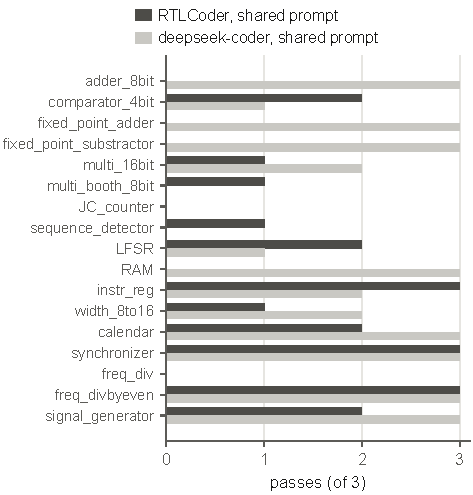
\includegraphics{fig_s_twin_a}
\caption{Fine-tuning twin, shared prompt}
\label{fig:s-twin-a}
\end{subfigure}\hfill
\begin{subfigure}[t]{3.15in}
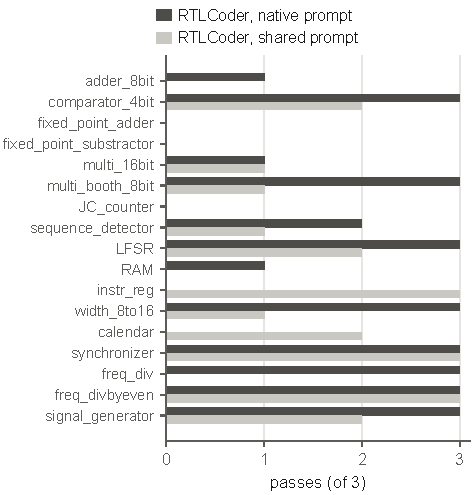
\includegraphics{fig_s_twin_b}
\caption{Prompt format, RTLCoder}
\label{fig:s-twin-b}
\end{subfigure}
\caption{The Twin run on the $17$ recoverable modules, passes of $3$, $T{=}0.5$.
(a)~Fine-tuning shows no net advantage at the shared prompt: $0$ wins, $13$
ties, $4$ losses (\texttt{adder\_8bit}, \texttt{fixed\_point\_adder},
\texttt{fixed\_point\_substractor}, \texttt{RAM}; \texttt{width\_8to16}, $1/3$
against $2/3$, counts as a tie). (b)~Prompt format has a modest, inconsistent
effect: native wins $3$ modules, shared $2$.}
\label{fig:s-twin}
\end{figure}

% ============================================================================
\section{Sets 1 and 3 in Detail}
\label{s:sets13}

\textbf{Scope and timeouts.} Set~1: of $1{,}512$ cells, $6$ ($0.4\%$) errored
as timeouts and are excluded: five on \texttt{RAM} with llama3.1
(\cond{sem\_escalate} replicates $1$ to $3$, \cond{sem\_escalate\_restart}
replicates $1$ and $3$) and one on \texttt{LIFObuffer} with deepseek-coder
(\cond{sem\_escalate\_restart}, replicate $2$). \texttt{RAM}/llama3.1 is $0/3$
under baseline and \cond{sem\_adv}, so counting the missing runs as failures
moves the recoverable rates to $47/153$ ($30.7\%$) and $54/153$ ($35.3\%$); no
conclusion changes. Set~3: of $612$ cells, $2$ ($0.3\%$) errored
(qwen2.5-coder:32b, one \texttt{comparator\_4bit} and one
\texttt{multi\_booth\_8bit}).

\textbf{Iteration budget.} \cond{baseline} and \cond{sem\_adv} were capped at
six iterations, the escalation policies at eight, the Twin baselines at eight.
On the recoverable band one \cond{sem\_escalate} and one
\cond{sem\_escalate\_restart} pass in Set~1 arrived only in iterations seven or
eight ($47/150$ becomes $46/150$, and $54/151$ becomes $53/151$, at a cap of
six), and none in Set~3; at an equal cap \cond{sem\_escalate\_restart} is
$53/151$ ($35.1\%$) against baseline's $54/153$ ($35.3\%$).

\begin{table}[!htbp]
\centering
\footnotesize
\caption{Set~1 passes by tier and condition ($3$ models, $N{=}3$). The
conditions differ only on the recoverable band.}
\label{tab:s-tier-pass}
\begin{tabular}{@{}l r rrrr@{}}
\toprule
Tier & Modules & \cond{baseline} & \cond{sem\_adv} & \cond{sem\_escalate} & \cond{sem\_esc\_restart} \\
\midrule
Ceiling     & 6  & 44/54   & 44/54   & 46/54   & 43/54 \\
Recoverable & 17 & 54/153  & 47/153  & 47/150  & 54/151 \\
Floor       & 19 & 11/171  & 12/171  & 11/171  & 11/170 \\
\midrule
Pooled      & 42 & 109/378 & 103/378 & 104/375 & 108/375 \\
Pooled, \%  &    & 28.8    & 27.2    & 27.7    & 28.8 \\
\bottomrule
\end{tabular}
\end{table}

\begin{table}[!htbp]
\centering
\footnotesize
\caption{Set~1 Verilator and Yosys calls per run by tier, and the cut of
\cond{sem\_escalate} against \cond{sem\_adv}: largest where baseline already
succeeds.}
\label{tab:s-tier-cost}
\begin{tabular}{@{}l r rr r@{}}
\toprule
Tier & Modules & \cond{sem\_adv} & \cond{sem\_escalate} & Cut, \% \\
\midrule
Ceiling     & 6  & 4.02 & 1.00 & 75.1 \\
Recoverable & 17 & 6.74 & 5.62 & 16.6 \\
Floor       & 19 & 7.28 & 6.54 & 10.1 \\
\midrule
Pooled      & 42 & 6.60 & 5.38 & 18.5 \\
\bottomrule
\end{tabular}
\end{table}

\begin{figure}[!htbp]
\centering
\begin{subfigure}[t]{3.15in}
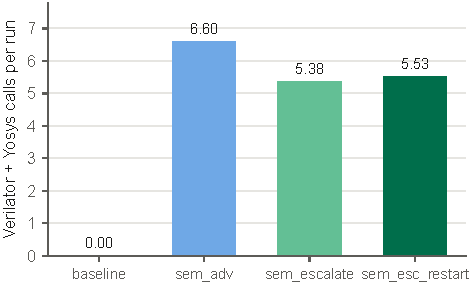
\includegraphics{fig_s_set1_calls}
\caption{Tool calls per run}
\label{fig:s-set1-a}
\end{subfigure}\hfill
\begin{subfigure}[t]{3.15in}
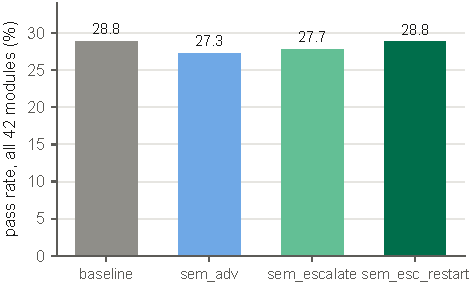
\includegraphics{fig_s_set1_pass}
\caption{Pass rate}
\label{fig:s-set1-b}
\end{subfigure}
\caption{Set~1, $1{,}512$ runs, pooled over all $42$ modules. (a)~Escalation
calls Verilator and Yosys less often than always-on interpretation. (b)~The
pooled pass rates lie within $1.6$ points of each other.}
\label{fig:s-set1-cost}
\end{figure}

\begin{table}[!htbp]
\centering
\footnotesize
\caption{Set~3, recoverable band, $T{=}0.1$: pass rate (\%) per model ($n{=}51$
per cell, except qwen2.5-coder:32b \cond{sem\_esc\_restart}, $n{=}49$) and the
pooled passes.}
\label{tab:s-set3}
\begin{tabular}{@{}l rrrr@{}}
\toprule
Model & \cond{baseline} & \cond{sem\_adv} & \cond{sem\_escalate} & \cond{sem\_esc\_restart} \\
\midrule
qwen2.5-coder:14b & 52.9 & 49.0 & 56.9 & 58.8 \\
gemma3:27b        & 37.3 & 45.1 & 37.3 & 33.3 \\
qwen2.5-coder:32b & 78.4 & 72.6 & 82.4 & 83.7 \\
\midrule
Pooled            & 86/153 & 85/153 & 90/153 & 88/151 \\
Pooled, \%        & 56.2 & 55.6 & 58.8 & 58.3 \\
\bottomrule
\end{tabular}
\end{table}

\textbf{Replicate trace (Set~3).} Of $153$ \cond{sem\_escalate} runs, $88$ passed
without escalating, $65$ escalated, and $2$ of those passed, both with
\cond{semantic\_fired}${=}0$, rescued by raw Verilator and Yosys feedback within
the first six iterations. No passing \cond{sem\_escalate} run had the interpreter
fire; for \cond{sem\_escalate\_restart} one of $88$ passing runs did, and seven of
\cond{sem\_adv}'s $85$. The net pooled escalation lead ($+4$ runs) comes from six
cells gaining seven runs in total against three cells losing one each. Set~3
tool calls on the recoverable band: $5.31$ (\cond{sem\_adv}) to $3.85$
(\cond{sem\_escalate}) per run, $27.6\%$.

\begin{table}[!htbp]
\centering
\footnotesize
\caption{Recoverable-band contrasts against baseline: points, (model, module)
cell bootstrap $95\%$ CI and sign-flip $p$
(\texttt{phase3/runner/posthoc\_checks.py}). None differs from baseline.}
\label{tab:s-posthoc}
\begin{tabular}{@{}l l r S[table-format=+1.1] S[table-format=+2.1]@{\ to\ }S[table-format=+1.1] r@{}}
\toprule
Run & Condition $-$ baseline & Passes & {$\Delta$} & \multicolumn{2}{c}{95\% CI} & $p$ \\
\midrule
Set~1 & \cond{sem\_adv}              & 47/153 vs 54/153 & -4.6 & -10.5 & +0.7 & 0.199 \\
Set~1 & \cond{sem\_escalate}         & 47/150 vs 54/153 & -4.7 & -10.7 & +0.0 & 0.148 \\
Set~1 & \cond{sem\_escalate\_restart} & 54/151 vs 54/153 & 0.0 & -4.6 & +4.6 & 1.000 \\
\addlinespace
Set~3 & \cond{sem\_adv}              & 85/153 vs 86/153 & -0.7 & -7.8 & +6.5 & 1.000 \\
Set~3 & \cond{sem\_escalate}         & 90/153 vs 86/153 & +2.6 & -1.3 & +7.2 & 0.404 \\
Set~3 & \cond{sem\_escalate\_restart} & 88/151 vs 86/153 & +2.0 & -2.6 & +7.2 & 0.596 \\
\bottomrule
\end{tabular}
\end{table}

% ============================================================================
\section{The API Study (Sets 4, 4b and 4c)}
\label{s:api}

\textbf{Design.} Pre-registered in \texttt{phase2/frontier/SET4\_PREREG.md}
(original and five dated amendments, each hashed before the calls it governs;
hash after the last amendment \texttt{CC23711D\ldots653B}). Models:
\texttt{gpt-4.1-mini-\allowbreak 2025-04-14} (pinned snapshot),
\texttt{gemini-2.5-flash} (\texttt{thinkingBudget} $0$) and
\texttt{claude-haiku-4-5-\allowbreak 20251001} (no extended thinking), selected as the most
capable non-reasoning model per provider under a cost rule; $T{=}0.1$;
\texttt{max\_tokens} $8{,}192$. Any reasoning token or reasoning content on any
call stops the provider; there were none. The engine is the Set~3 runner with
only the model call replaced; pass detection is
\texttt{detect\_outcome(log, benchmark="rtllm")}. Toolchain: oss-cad-suite
20260917 in WSL, matched to the cluster build (Yosys~0.69+71, Verilator~5.053,
Icarus~14.0); on $140$ saved Set~3 candidates it reproduces the cluster verdicts
($\SetFourParitySim$ pass/fail, $\SetFourParityInterp$ interpreter outputs).
Every call logs provider-reported tokens, the returned model version, request
and response identifiers and cost; truncations: $0$ in every set.

\textbf{Deviations, disclosed.} (1)~A fourth model (Kimi K2.6) stopped at its
smoke test with \texttt{reasoning\_tokens}${=}1$ and was dropped by decision; a
third ceiling model at a forced $T{=}0.6$ would add no information.
(2)~OpenAI's \texttt{system\_fingerprint} changed during the run
($\SetFourFingerprintMain$ and $\SetFourFingerprintOther$ calls) for the same
snapshot. (3)~Set~4b first stopped at caps set from a pilot projection that
underestimated floor cost; completion runs resumed from the master logs without
re-running any completed run. Claude Haiku~4.5 is at
$\SetFourBHaikuValid/\SetFourBPlanned$: $\SetFourBHaikuErrored$ runs errored on
an exhausted account credit (HTTP 400) and are pending; they are excluded, and
every number here is regenerated by script if they are completed.

% BEGIN GENERATED TABLES
\begin{table}[!htbp]
\centering
\footnotesize
\caption{Set~4, recoverable band ($17$ modules, $N{=}3$): passes per condition, with the pooled rate and its Wilson $95\%$ CI. All three models are at or near ceiling.}
\label{tab:s-set4-pass}
\begin{tabular}{@{}l rrrr@{}}
\toprule
Model & \cond{baseline} & \cond{sem\_adv} & \cond{sem\_escalate} & \cond{sem\_esc\_restart} \\
\midrule
GPT-4.1 mini & 50/51 & 49/51 & 48/51 & 48/51 \\
Gemini 2.5 Flash & 51/51 & 51/51 & 51/51 & 51/51 \\
Claude Haiku 4.5 & 51/51 & 51/51 & 51/51 & 51/51 \\
\midrule Pooled & 152/153 & 151/153 & 150/153 & 150/153 \\
Pooled, \% [CI] & 99.3 [96.4, 99.9] & 98.7 [95.4, 99.6] & 98.0 [94.4, 99.3] & 98.0 [94.4, 99.3] \\
\bottomrule
\end{tabular}
\end{table}

\begin{table}[!htbp]
\centering
\footnotesize
\caption{Set~4: condition minus baseline (points), (model, module) cell bootstrap $95\%$ CI and sign-flip $p$. No contrast differs from baseline.}
\label{tab:s-set4-contrast}
\begin{tabular}{@{}l rr rr rr@{}}
\toprule
 & \multicolumn{2}{c}{\cond{sem\_adv}} & \multicolumn{2}{c}{\cond{sem\_escalate}} & \multicolumn{2}{c}{\cond{sem\_esc\_restart}} \\ \cmidrule(lr){2-3}\cmidrule(lr){4-5}\cmidrule(l){6-7} Scope & $\Delta$ [CI] & $p$ & $\Delta$ [CI] & $p$ & $\Delta$ [CI] & $p$ \\
\midrule
Pooled (51 cells) & $-$0.7 [$-$2.0, +0.0] & 1.000 & $-$1.3 [$-$3.9, +0.0] & 1.000 & $-$1.3 [$-$3.9, +0.0] & 1.000 \\
GPT-4.1 mini & $-$2.0 [$-$5.9, +0.0] & 1.000 & $-$3.9 [$-$11.8, +0.0] & 1.000 & $-$3.9 [$-$11.8, +0.0] & 1.000 \\
Gemini 2.5 Flash & +0.0 [+0.0, +0.0] & 1.000 & +0.0 [+0.0, +0.0] & 1.000 & +0.0 [+0.0, +0.0] & 1.000 \\
Claude Haiku 4.5 & +0.0 [+0.0, +0.0] & 1.000 & +0.0 [+0.0, +0.0] & 1.000 & +0.0 [+0.0, +0.0] & 1.000 \\
\bottomrule
\end{tabular}
\end{table}

\begin{table}[!htbp]
\centering
\footnotesize
\caption{Set~4 mechanism trace. \cond{sem\_adv}: runs where the interpreter fired, and passes with it firing (in brackets: fired on an iteration before the passing one). Escalation conditions: escalated runs (of which passed). Last three columns: Verilator and Yosys calls per run and the cut of \cond{sem\_escalate} against \cond{sem\_adv}.}
\label{tab:s-set4-trace}
\begin{tabular}{@{}l rrrr rrr@{}}
\toprule
Model & \makecell{fired\\runs} & \makecell{passes\\fired} & \makecell{\cond{sem\_esc.}\\escalated} & \makecell{\cond{sem\_esc\_rst.}\\escalated} & \makecell{calls\\\cond{sem\_adv}} & \makecell{calls\\\cond{sem\_esc.}} & \makecell{cut\\\%} \\
\midrule
GPT-4.1 mini & 5 & 5 (0) & 3 (0) & 3 (0) & 2.39 & 0.71 & 70.5 \\
Gemini 2.5 Flash & 6 & 6 (1) & 0 (0) & 1 (1) & 2.22 & 0.00 & 100.0 \\
Claude Haiku 4.5 & 9 & 9 (4) & 2 (2) & 1 (1) & 2.25 & 0.08 & 96.5 \\
\midrule Pooled & 20 & 20 (5) & 5 (2) & 5 (2) & 2.29 & 0.26 & 88.6 \\
\bottomrule
\end{tabular}
\end{table}

\begin{table}[!htbp]
\centering
\footnotesize
\caption{Set~4 cost in INR per run and per passing run (USD $\times 96 \times 1.18$, list prices).}
\label{tab:s-set4-cost}
\begin{tabular}{@{}l rr rr rr rr@{}}
\toprule
 & \multicolumn{2}{c}{\cond{baseline}} & \multicolumn{2}{c}{\cond{sem\_adv}} & \multicolumn{2}{c}{\cond{sem\_escalate}} & \multicolumn{2}{c}{\cond{sem\_esc\_restart}} \\ \cmidrule(lr){2-3}\cmidrule(lr){4-5}\cmidrule(lr){6-7}\cmidrule(l){8-9} Model & run & pass & run & pass & run & pass & run & pass \\
\midrule
GPT-4.1 mini & 0.112 & 0.114 & 0.127 & 0.132 & 0.158 & 0.168 & 0.158 & 0.168 \\
Gemini 2.5 Flash & 0.245 & 0.245 & 0.236 & 0.236 & 0.224 & 0.224 & 0.233 & 0.233 \\
Claude Haiku 4.5 & 0.506 & 0.506 & 0.473 & 0.473 & 0.478 & 0.478 & 0.495 & 0.495 \\
\bottomrule
\end{tabular}
\end{table}

\begin{table}[!htbp]
\centering
\footnotesize
\caption{Set~4b coverage, of $228$ planned runs per model. Errored runs failed on an exhausted account credit, cost nothing, and are excluded (pending).}
\label{tab:s-set4b-cov}
\begin{tabular}{@{}l rrr@{}}
\toprule
Model & valid & \makecell{errored\\(pending)} & not run \\
\midrule
GPT-4.1 mini & 228 & 0 & 0 \\
Gemini 2.5 Flash & 228 & 0 & 0 \\
Claude Haiku 4.5 & 143 & 85 & 0 \\
\bottomrule
\end{tabular}
\end{table}

\begin{table}[!htbp]
\centering
\footnotesize
\caption{Set~4b per floor module: baseline passes of $3$ with the tier this model puts the module in (Q1; C ceiling, R recoverable, F floor), and passes over all valid runs of all four conditions (Q4). --: not run (measured values only; projections: \cref{tab:s-proj}).}
\label{tab:s-set4b-q1}
\begin{tabular}{@{}l rr rr rr@{}}
\toprule
 & \multicolumn{2}{c}{GPT-4.1 mini} & \multicolumn{2}{c}{Gemini 2.5 Flash} & \multicolumn{2}{c}{Claude Haiku 4.5} \\ \cmidrule(lr){2-3}\cmidrule(lr){4-5}\cmidrule(l){6-7} Module & Q1 & Q4 & Q1 & Q4 & Q1 & Q4 \\
\midrule
\texttt{accu} & 3/3 C & 12/12 & 3/3 C & 12/12 & 3/3 C & 12/12 \\
\texttt{adder\_16bit} & 3/3 C & 12/12 & 3/3 C & 12/12 & 3/3 C & 12/12 \\
\texttt{adder\_32bit} & 3/3 C & 12/12 & 3/3 C & 12/12 & 3/3 C & 11/12 \\
\texttt{adder\_bcd} & 3/3 C & 12/12 & 3/3 C & 12/12 & 3/3 C & 12/12 \\
\texttt{adder\_pipe\_64bit} & 0/3 F & 2/12 & 0/3 F & 0/12 & 0/3 F & 4/12 \\
\texttt{alu} & 0/3 F & 0/12 & 0/3 F & 3/12 & 0/3 F & 0/12 \\
\texttt{barrel\_shifter} & 1/3 R & 1/12 & 3/3 C & 12/12 & -- & -- \\
\texttt{counter\_12} & 3/3 C & 12/12 & 3/3 C & 12/12 & -- & -- \\
\texttt{div\_16bit} & 0/3 F & 0/12 & 0/3 F & 0/12 & 2/3 R & 6/12 \\
\texttt{float\_multi} & 2/3 R & 4/12 & 1/3 R & 4/12 & 1/3 R & 1/11 \\
\texttt{freq\_divbyfrac} & 0/3 F & 0/12 & 0/3 F & 0/12 & 0/3 F & 0/12 \\
\texttt{fsm} & 3/3 C & 11/12 & 3/3 C & 11/12 & -- & -- \\
\texttt{LIFObuffer} & 3/3 C & 12/12 & 3/3 C & 9/12 & -- & -- \\
\texttt{multi\_pipe\_4bit} & 3/3 C & 12/12 & 0/3 F & 8/12 & 3/3 C & 12/12 \\
\texttt{multi\_pipe\_8bit} & 0/3 F & 0/12 & 1/3 R & 2/12 & 3/3 C & 12/12 \\
\texttt{parallel2serial} & 0/3 F & 1/12 & 1/3 R & 5/12 & 3/3 C & 12/12 \\
\texttt{pulse\_detect} & 0/3 F & 0/12 & 3/3 C & 8/12 & -- & -- \\
\texttt{serial2parallel} & 3/3 C & 12/12 & 3/3 C & 11/12 & -- & -- \\
\texttt{traffic\_light} & 2/3 R & 4/12 & 0/3 F & 4/12 & -- & -- \\
\bottomrule
\end{tabular}
\end{table}

\begin{table}[!htbp]
\centering
\footnotesize
\caption{Set~4b, Q2: the interpreter on floor failures. Passes with a directive delivered before the passing iteration, and those in cells whose baseline was $0/3$ (each traced; none attributable to the directive).}
\label{tab:s-set4b-q2}
\begin{tabular}{@{}l rrrrrrr@{}}
\toprule
Condition & runs & fails & \makecell{fails\\fired} & passes & \makecell{directive\\before pass} & \makecell{of which\\baseline $0/3$} & escalated \\
\midrule
\cond{baseline} & 150 & 61 & 0 & 89 & 0 & 0 & -- \\
\cond{sem\_adv} & 150 & 68 & 37 & 82 & 11 & 3 & -- \\
\cond{sem\_escalate} & 150 & 63 & 33 & 87 & 1 & 0 & 84 \\
\cond{sem\_esc\_restart} & 149 & 57 & 33 & 92 & 0 & 0 & 75 \\
\bottomrule
\end{tabular}
\end{table}

\begin{table}[!htbp]
\centering
\footnotesize
\caption{Set~4b, Q3: condition minus baseline on cells whose baseline was below $3/3$ (points, cell bootstrap $95\%$ CI, sign-flip $p$). No contrast is significant.}
\label{tab:s-set4b-q3}
\begin{tabular}{@{}l r rr rr rr@{}}
\toprule
 & & \multicolumn{2}{c}{\cond{sem\_adv}} & \multicolumn{2}{c}{\cond{sem\_escalate}} & \multicolumn{2}{c}{\cond{sem\_esc\_restart}} \\ \cmidrule(lr){3-4}\cmidrule(lr){5-6}\cmidrule(l){7-8} Scope & cells & $\Delta$ [CI] & $p$ & $\Delta$ [CI] & $p$ & $\Delta$ [CI] & $p$ \\
\midrule
Pooled & 24 & $-$2.8 [$-$15.3, +11.1] & 0.848 & +1.4 [$-$11.1, +13.9] & 1.000 & +8.3 [$-$6.9, +23.6] & 0.407 \\
GPT-4.1 mini & 10 & $-$10.0 [$-$23.3, +0.0] & 0.505 & $-$3.3 [$-$20.0, +13.3] & 1.000 & $-$13.3 [$-$33.3, +3.3] & 0.372 \\
Gemini 2.5 Flash & 9 & +3.7 [$-$18.5, +33.3] & 1.000 & +14.8 [$-$3.7, +37.0] & 0.374 & +33.3 [+11.1, +55.6] & 0.062 \\
Claude Haiku 4.5 & 5 & +0.0 [$-$26.7, +33.3] & 1.000 & $-$13.3 [$-$26.7, +0.0] & 0.496 & +6.7 [$-$20.0, +40.0] & 1.000 \\
\bottomrule
\end{tabular}
\end{table}

\subsection*{Haiku projection (to be replaced by measured runs)}
Claude Haiku~4.5 is measured on 12 of 19 floor modules. Only two places in the paper need a complete Haiku column, the floor heat map and the count of modules at ceiling for all three models; there, each missing (module, condition) cell is projected and marked with a dagger. Each projection starts from the mean pass rate of GPT-4.1 mini and Gemini 2.5 Flash on that cell and shifts it on the logit scale by Haiku's mean logit difference from those two models over the 47 cells all three measured in full (empirical logits with one half added to each count, so that $0/3$ and $3/3$ stay finite): $+0.72$ logits, Haiku being the stronger. A mean rate of exactly $0$ or $1$ stays there. The range is the lower to the higher of the two other models' rates. Every observed conclusion in the paper uses measured runs only, and \texttt{make\_numbers\_set4.py} replaces each projection once the runs are completed. Inputs, method and outputs: \texttt{phase2/frontier/evidence/set4b\_haiku\_projection.json}.

\begin{table}[!htbp]
\centering
\footnotesize
\caption{Projected Claude Haiku~4.5 passes of $3$ per missing cell, with the range spanned by GPT-4.1 mini and Gemini 2.5 Flash in brackets. --: measured (\texttt{float\_multi} lacks one \cond{sem\_esc\_restart} run; its value is the projected expectation for a full cell).}
\label{tab:s-proj}
\begin{tabular}{@{}l rrrr@{}}
\toprule
Module & \cond{baseline} & \cond{sem\_adv} & \cond{sem\_escalate} & \cond{sem\_esc\_restart} \\
\midrule
\texttt{barrel\_shifter} & 2.4 [1, 3] & 2.0 [0, 3] & 2.0 [0, 3] & 2.0 [0, 3] \\
\texttt{counter\_12} & 3.0 [3, 3] & 3.0 [3, 3] & 3.0 [3, 3] & 3.0 [3, 3] \\
\texttt{float\_multi} & -- & -- & -- & 1.5 [0, 2] \\
\texttt{fsm} & 3.0 [3, 3] & 3.0 [3, 3] & 3.0 [3, 3] & 2.4 [2, 2] \\
\texttt{LIFObuffer} & 3.0 [3, 3] & 2.4 [1, 3] & 2.7 [2, 3] & 3.0 [3, 3] \\
\texttt{pulse\_detect} & 2.0 [0, 3] & 0.9 [0, 1] & 1.5 [0, 2] & 1.5 [0, 2] \\
\texttt{serial2parallel} & 3.0 [3, 3] & 2.7 [2, 3] & 3.0 [3, 3] & 3.0 [3, 3] \\
\texttt{traffic\_light} & 1.5 [0, 2] & 0.0 [0, 0] & 2.4 [2, 2] & 1.5 [0, 2] \\
\bottomrule
\end{tabular}
\end{table}

% END GENERATED TABLES

\textbf{Q4 and the oracle audit.} Of the $\SetFourBAllThreeModules$ modules all
three models ran, only \SetFourBQFour{} fails in every run by every model under
every condition (\cref{s:freq}). \texttt{alu} fails for GPT-4.1 mini and
Claude Haiku~4.5 but Gemini~2.5 Flash passes it in $\SetFourBAluGemini$ runs, so
its testbench can be passed as written; it remains a feedback-poor testbench (one
error line for any mismatch over $17$ opcodes), and the Gemini passes came after
simulation and tool feedback with no directive before the pass.

\textbf{Set 4c.} A Gemini~2.5 Pro (reasoning) run on the residual floor was
closed by its pre-registered stop rule on its first run (thinking tokens above
the budget; the answer cut off) with $0$ of $18$ runs completed; no results are
reported.

% ============================================================================
\section{freq\_divbyfrac in Detail}
\label{s:freq}

\textbf{Specification} (RTLLM \texttt{design\_description.txt}, lines 16 to 20,
verbatim): ``For 3.5x division: The counter cycles through 7 half clock steps
(MUL2\_DIV\_CLK = 7). It generates one divided clock pulse on the positive edge
of clk, and another adjusted pulse on the negative edge of clk. The
negative-edge pulse extends the output by half a source clock cycle, so the
final output has the required 3.5x division period. In each divided clock
period, clk\_div keeps high for the first 3 half clock steps and keeps low for
the next 4 half clock steps.''

\textbf{Testbench} (\texttt{testbench.v}): the clock toggles every $5$\,ns
(line 15) and starts high (line 22); reset is released at $t{=}10$\,ns (line 24),
in the same time step as a rising edge; $20$ checks run every $5$\,ns from
$t{=}15$\,ns (lines 31 to 45), each comparing \texttt{clk\_div} with the value set
on the previous iteration (lines 33 to 44). The expected sequence over the $20$
checks is \texttt{11100001110000111000}: three high and four low half steps,
repeating.

\textbf{The reference, logged} (\texttt{phase2/frontier/set4c.py refcheck}). The
original testbench with one added \texttt{\$strobe} of the counter and the two
intermediate clocks at every clock edge shows that the counter advances once per
rising edge ($0$ to $6$, never on a falling edge), so it wraps every $14$ half
steps, and \texttt{clk\_div} has a period of $7$ half steps (high $3$, low $4$):
two output periods per counter wrap. The reference passes. Spec line 17 says the
counter ``cycles through 7 half clock steps''; the reference's counter cycles
through $7$ rising edges.

\textbf{The candidates} (\texttt{set4c.py trace}). The original testbench with one
added \texttt{\$display} at each check (same statement position, so the same
event ordering) was run on the final candidate of each of the $36$ Set~4b runs
(\cref{tab:s-freq}).

\begin{table}[!htbp]
\centering
\footnotesize
\caption{\texttt{freq\_divbyfrac} final candidates against the expected
sequence: none is a phase-shifted copy; most have about twice the period.}
\label{tab:s-freq}
\begin{tabularx}{\linewidth}{@{}l X@{}}
\toprule
Item & Result \\
\midrule
Reference & passes; $20/20$ at shift $0$, $14/19$ at $\pm1$ check, $8/18$ at $\pm2$ \\
Candidates that compile & $34$ of $36$ \\
Match at shift $0$ & $0$ \\
Pure shift of the expected sequence & $0$ \\
First mismatching check & check~3 (\texttt{clk\_div=1}, expected $0$) in $32$; check~0 in $2$ \\
First high phase ($32$ starting high) & $4$ to $20$ half steps (H4 $5$, H5 $3$, H6 $6$, H7 $7$, H9 $3$, H11 $3$, H13 $4$, H20 $1$) \\
Typical traces & \texttt{H6 L7 H7}, \texttt{H7 L7 H6}: a period of about $13$ to $14$ half steps \\
\bottomrule
\end{tabularx}
\end{table}

\textbf{Reading.} No candidate fails by a phase offset that a more lenient
testbench would forgive. This is not a testbench defect; the specification's own
description of the counter (``7 half clock steps'') does not match its reference
design (seven rising edges, two output periods per wrap), in our reading; and
the models fail on period and duty cycle, producing roughly twice the specified
period. The same-time-step reset release is a minor robustness weakness of the
testbench that did not cause these failures. The spec text and testbench lines
are collected in \texttt{phase2/frontier/FREQ\_DIVBYFRAC\_AUDIT.md}.

% ============================================================================
\section{The MPSoC Case Study in Full}
\label{s:p3}

\subsection{Substrate}

The MPSoC has a five-stage RV32 core, a network interface (packetiser,
depacketiser, asynchronous FIFOs) and a virtual-channel wormhole mesh router,
built as a $2{\times}2$ mesh ($4$ routers) and a $3{\times}3$ mesh ($9$ routers)
that share $28$ of $33$ router leaf files. Only compile-level changes were made
for the open-source flow (redeclarations, nested comments, and Vivado-style
implicit trailing ports reproduced with identical binding). Synthesis of the top
reports $63$ latch inferences across $12$ module definitions and then aborts on
a one-bit register that tests \texttt{clr | reset} inside an asynchronous-reset
block (\cref{tab:s-p3-prop}). Repairing the eight task leaves turns the abort
into a pass; $122$ latch cells remain in five modules outside the repair set.
The top-level testbench executes two instructions and never exercises the
network, so it is a weak oracle and top-level claims are structural.

\begin{table}[!htbp]
\centering
\footnotesize
\caption{Leaf defects composed into the real designs. Latch cells scale with
the router count ($6{,}480/2{,}880 = 9/4$) while Yosys prints the same two
messages; repairing the task leaves restores synthesis. For the MPSoC, $122$
latch cells remain in five modules outside the repair set, so its bound is
restored synthesis, not a latch-free design.}
\label{tab:s-p3-prop}
\begin{tabular}{@{}l rrr@{}}
\toprule
 & $2{\times}2$ mesh & $3{\times}3$ mesh & MPSoC top \\
\midrule
Yosys latch messages, as written          & 2 & 2 & 63 \\
Latch cells (abort-causing file excluded) & 2,880 & 6,480 & 269 \\
Top-level synthesis, as written           & aborts & aborts & aborts \\
Top-level synthesis, task leaves repaired & pass & pass & pass \\
Latch cells, task leaves repaired         & 0 & 0 & 122 \\
\bottomrule
\end{tabular}
\end{table}

\subsection{The v3 layer}

Real logs exposed three kinds of wrong advice (an unused clock got the gating
template, \texttt{if (clk)} in a combinational block, which builds a
clock-gated latch; a legitimately part-unused instruction bus was turned into
``gate the output on this bus''; one file holding several modules produced
advice for the wrong module) and three silences (the asynchronous-reset abort
names no signal; a truncation whose operand is an expression was dropped; a loop
only Verilator reports never reached the model). v3 fixes these additively
(\cref{s:interp}). A live drift gate runs the interpreter on fresh tool
output before any GPU time; it caught a latch-message format change between
Yosys~0.33 and 0.69.

\subsection{Experiment details}

\textbf{Conditions.} As in the main text; all receive simulation feedback and
share six model calls, the same prompt and identically filtered raw tool text;
every candidate is fully evaluated (simulation, lint, synthesis). The
\cond{sem\_esc\_restart} (v3) gate message is ``the design simulates correctly
but fails synthesis sign-off''. \cond{baseline\_gate} logs \texttt{would\_fire}
(v3 fires on at least one RTL the alarm was given on) and
\texttt{would\_fire\_final} (on the returned RTL), never fed back.

\textbf{Pre-registration and freeze.} \texttt{phase3/evidence/PREREG\_FINAL.md}
(SHA-256 \texttt{1b6eb915\ldots cc63}) was frozen with the runner, interpreter,
prompt and task files (\texttt{FREEZE\_FINAL.md}); every new run records their
hashes, its node, its toolchain and its model digest. The six model digests were
identical before and after the $32$B pull. Protocol fields are identical across
all $1{,}386$ cluster runs. The API rows were pre-registered separately
(\texttt{phase2/frontier/p3\_api/P3\_API\_PREREG.md}) and ran the same runner
code (SHA-256 \texttt{119611fe\ldots6a36}); a mock parity check confirmed that
the (system, user) texts sent are byte-identical to the Ollama path ($96$ of
$96$ requests per provider).

\textbf{Inference backend.} The control arm's Ollama server fell back to Vulkan
after CUDA discovery timed out (same H200 GPU, all layers on the GPU). On
sim-visible tasks the first prompt of \cond{baseline\_gate} and \cond{baseline}
is byte-identical ($90$ of $90$); the first responses are byte-identical in
$112$ of $270$ cross-arm pairs ($41\%$) against $37$ of $90$ ($41\%$) for two
baseline replicates; first-call simulation pass $42/90$ against $44/90$.

\textbf{Metrics.} Loop pass: the loop testbench passes. Sign-off clean: the
sign-off testbench passes and Yosys synthesises the module with no latch and no
loop and Verilator reports none of \cond{MULTIDRIVEN}, \cond{UNOPTFLAT},
\cond{LATCH}, \cond{WIDTHTRUNC}. Signed off defective: loop pass and not sign-off
clean. Loop-clean (\texttt{clean\_pass} in the code): the loop testbench with the
same structural rule. Silent structural pass (first write-up): loop pass and not
structurally clean.

\subsection{Results tables}

\begin{table}[!htbp]
\centering
\footnotesize
\caption{Outcome per condition, six models, $198$ runs each, in percent
(sign-off clean with its Wilson $95\%$ CI).}
\label{tab:s-p3-pooled}
\begin{tabular}{@{}l r rc r r r r@{}}
\toprule
Condition & \makecell[r]{Loop\\pass} & \makecell[r]{Sign-off\\clean} & \makecell{95\%\\CI} & \makecell[r]{Loop-\\clean} &
  \makecell[r]{Signed off\\defective} & \makecell[r]{Silent\\struct.} & \makecell[r]{Tokens\\per run} \\
\midrule
\cond{baseline}               & 85 & 22 & 17--28 & 23 & 63 & 62 & 1,425 \\
\cond{raw\_adv}               & 65 & 53 & 46--59 & 59 & 12 & 6  & 4,396 \\
\cond{sem\_adv} (v2)          & 71 & 63 & 56--69 & 68 & 8  & 3  & 3,831 \\
\cond{sem\_adv} (v3)          & 74 & 67 & 60--73 & 74 & 8  & 1  & 3,377 \\
\cond{sem\_esc\_restart} (v3) & 85 & 72 & 65--78 & 80 & 13 & 5  & 3,798 \\
\cond{baseline\_gate}         & 67 & 52 & 45--59 & 56 & 15 & 11 & 3,835 \\
\bottomrule
\end{tabular}
\end{table}

\textbf{By stratum.} Sign-off clean on the six sim-silent tasks ($n{=}108$):
baseline $0$, raw text $64$, v2 $83$, v3 $86$, escalation $86$, alarm $61$; on
the five sim-visible tasks ($n{=}90$): $43$, $40$, $41$, $46$, $56$ and $42$.

\begin{table}[!htbp]
\centering
\footnotesize
\caption{Pre-registered primary contrasts by stratum, six models (all rows,
including contrast~3's strata): points, cell bootstrap $95\%$ CI, sign-flip $p$,
runs only A or only B got right.}
\label{tab:s-p3-primary}
\begin{tabular}{@{}l l S[table-format=+2.1] S[table-format=+2.1]@{\ to\ }S[table-format=+2.1] r r@{}}
\toprule
Contrast (A $-$ B) & Tasks & {$\Delta$} & \multicolumn{2}{c}{95\% CI} & $p$ & A/B only \\
\midrule
1. \cond{sem\_esc\_restart} $-$ \cond{baseline\_gate} & all & +19.7 & +11.1 & +29.3 & $<$0.001 & 42/3 \\
   & \quad sim-silent  & +23.1 & +11.1 & +37.0 & 0.002 & 27/2 \\
   & \quad sim-visible & +15.6 & +4.4  & +27.8 & 0.022 & 15/1 \\
\addlinespace
2. \cond{sem\_adv} (v3) $-$ \cond{baseline\_gate} & all & +14.6 & +3.0 & +26.3 & 0.021 & 43/14 \\
   & \quad sim-silent  & +23.1 & +6.5  & +39.8 & 0.014 & 31/6 \\
   & \quad sim-visible & +4.4  & -11.1 & +20.0 & 0.688 & 12/8 \\
\addlinespace
3. \cond{baseline\_gate} $-$ \cond{raw\_adv} & all & -0.5 & -9.1 & +8.1 & 1.000 & 16/17 \\
   & \quad sim-silent  & -2.8 & -13.0 & +7.4  & 0.738 & 6/9 \\
   & \quad sim-visible & +2.2 & -11.1 & +15.6 & 0.882 & 10/8 \\
\addlinespace
4. \cond{baseline\_gate} $-$ \cond{baseline} & sim-visible & -1.1 & -4.4 & +2.2 & 1.000 & 2/3 \\
\bottomrule
\end{tabular}
\end{table}

\begin{table}[!htbp]
\centering
\footnotesize
\caption{Primary contrasts (all tasks) under the pre-declared processor-level
sensitivity (\texttt{Address\_select} signed off by its loop testbench) and
under loop-clean: points and $95\%$ CI. Both give the same reading.}
\label{tab:s-p3-sens}
\begin{tabular}{@{}l S[table-format=+2.1] S[table-format=+2.1]@{\ to\ }S[table-format=+2.1] S[table-format=+2.1] S[table-format=+2.1]@{\ to\ }S[table-format=+2.1]@{}}
\toprule
 & \multicolumn{3}{c}{Processor-level view} & \multicolumn{3}{c}{Loop-clean} \\
\cmidrule(lr){2-4}\cmidrule(l){5-7}
Contrast & {$\Delta$} & \multicolumn{2}{c}{95\% CI} & {$\Delta$} & \multicolumn{2}{c}{95\% CI} \\
\midrule
1. \cond{sem\_esc\_restart} $-$ \cond{baseline\_gate}     & +24.2 & +14.6 & +34.3 & +23.7 & +14.1 & +33.8 \\
2. \cond{sem\_adv} (v3) $-$ \cond{baseline\_gate}         & +19.7 & +7.6  & +32.3 & +17.7 & +5.1  & +30.3 \\
3. \cond{baseline\_gate} $-$ \cond{raw\_adv}              & -3.0  & -12.1 & +6.1  & -3.0  & -12.1 & +6.1 \\
4. \cond{baseline\_gate} $-$ \cond{baseline} (sim-visible) & -2.2 & -7.8  & +3.3  & -2.2  & -7.8  & +3.3 \\
\bottomrule
\end{tabular}
\end{table}

\begin{table}[!htbp]
\centering
\footnotesize
\caption{\cond{baseline\_gate}: where the bare verdict was not enough (v3
interpretation logged, never fed back). \texttt{would\_fire}: v3 fires on an RTL
the alarm was given on; final: on the returned RTL.}
\label{tab:s-p3-wouldfire}
\begin{tabular}{@{}l rrrrr@{}}
\toprule
Task & Runs & \makecell[r]{Not sign-off\\clean} & \makecell[r]{with\\\texttt{would\_fire}} & \makecell[r]{with \texttt{would\_}\\\texttt{fire\_final}} & \makecell[r]{Clean with\\\texttt{would\_fire}} \\
\midrule
\texttt{Address\_select}   & 18 & 18 & 18 & 10 & 0 \\
\texttt{MuxPC}             & 18 & 3  & 3  & 0  & 15 \\
\texttt{execute\_mux}      & 18 & 6  & 6  & 0  & 12 \\
\texttt{mem\_wb\_mux}      & 18 & 9  & 9  & 3  & 9 \\
\texttt{mux3}              & 18 & 6  & 6  & 0  & 12 \\
\texttt{ni\_flit\_pack}    & 18 & 14 & 14 & 6  & 4 \\
\texttt{noc\_xbar4}        & 18 & 9  & 9  & 0  & 9 \\
\texttt{register\_1bit}    & 18 & 8  & 8  & 6  & 10 \\
\texttt{register\_32bit}   & 18 & 4  & 4  & 0  & 14 \\
\texttt{register\_4bit}    & 18 & 3  & 3  & 0  & 15 \\
\texttt{riscv\_alu\_flags} & 18 & 15 & 15 & 13 & 3 \\
\midrule
All                        & 198 & 95 & 95 & 38 & 103 \\
\bottomrule
\end{tabular}
\end{table}

\textbf{By model.} Escalation minus the alarm: $+39.4$ points on llama3.2:3b
($19/33$ against $6/33$) and $+33.3$ on gemma3:4b ($17/33$ against $6/33$), Holm
$p{=}0.006$ each; $+12.1$ (deepseek-coder:6.7b), $+18.2$ (qwen2.5-coder:7b),
$+9.1$ (llama3.1:8b) and $+6.1$ (qwen2.5-coder:14b), none significant after Holm
correction (\cref{fig:s-p3-models}). By task it is positive on ten of
eleven and zero on \texttt{noc\_xbar4}; none survives Holm correction across
eleven.

\begin{figure}[!htbp]
\centering
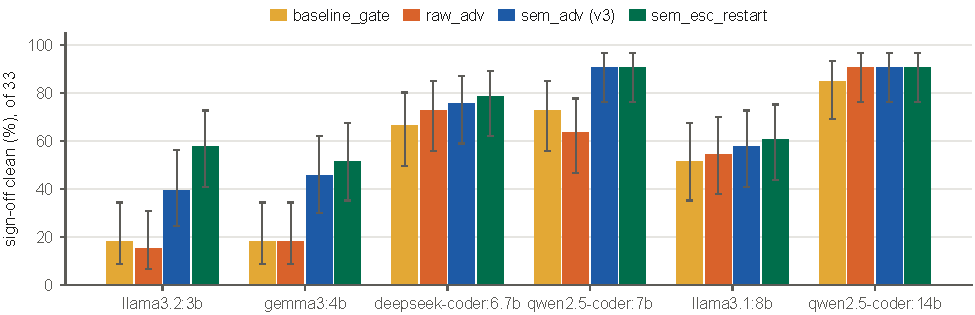
\includegraphics{fig_s_p3_models}
\caption{Sign-off clean per model under the alarm alone, raw tool text, v3 and
escalation ($33$ runs per bar, Wilson $95\%$ CI). Escalation leads for every
model, most on the two smallest.}
\label{fig:s-p3-models}
\end{figure}

\begin{table}[!htbp]
\centering
\footnotesize
\caption{Re-stated contrasts on sign-off clean, six models: points, cell
bootstrap $95\%$ CI and sign-flip $p$, with the loop-clean point estimate.}
\label{tab:s-p3-restated}
\begin{tabular}{@{}l l S[table-format=+2.1] S[table-format=+2.1]@{\ to\ }S[table-format=+2.1] r S[table-format=+2.1]@{}}
\toprule
A $-$ B & Tasks & {$\Delta$} & \multicolumn{2}{c}{95\% CI} & $p$ & {Loop-clean} \\
\midrule
\cond{sem\_adv} (v3) $-$ \cond{raw\_adv}          & all         & +14.1 & +3.5 & +24.7 & 0.014 & +14.6 \\
                                                 & \quad sim-silent  & +20.4 & +5.6 & +35.2 & 0.016 & +16.7 \\
                                                 & \quad sim-visible & +6.7  & -7.8 & +21.1 & 0.474 & +12.2 \\
\cond{sem\_adv} (v2) $-$ \cond{raw\_adv}          & all         & +10.1 & +2.0 & +18.7 & 0.030 & +9.1 \\
\cond{sem\_adv} (v3) $-$ \cond{sem\_adv} (v2)     & all         & +4.0  & -4.0 & +12.1 & 0.408 & +5.6 \\
\cond{sem\_esc\_restart} $-$ \cond{sem\_adv} (v3) & all         & +5.1  & -2.0 & +12.6 & 0.255 & +6.1 \\
\cond{sem\_esc\_restart} $-$ \cond{raw\_adv}      & all         & +19.2 & +9.6 & +28.8 & $<$0.001 & +20.7 \\
\cond{sem\_esc\_restart} $-$ \cond{baseline}      & sim-visible & +14.4 & +3.3 & +27.8 & 0.048 & +23.3 \\
\bottomrule
\end{tabular}
\end{table}

\begin{table}[!htbp]
\centering
\footnotesize
\caption{Cost per condition, six models. Tool rounds: model calls whose prompt
carried tool feedback. v3 needs the fewest tokens per sign-off clean run.}
\label{tab:s-p3-cost}
\begin{tabular}{@{}l rrrrr@{}}
\toprule
Condition & \makecell[r]{Calls\\per run} & \makecell[r]{Tool rounds\\per run} & \makecell[r]{Tokens\\per run} &
  \makecell[r]{Tokens per\\sign-off clean} & \makecell[r]{Clean by\\call 1, \%} \\
\midrule
\cond{baseline}               & 1.34 & 0.00 & 1,425 & 6,562 & 15 \\
\cond{raw\_adv}               & 3.27 & 3.27 & 4,396 & 8,370 & 41 \\
\cond{sem\_adv} (v2)          & 2.83 & 2.83 & 3,831 & 6,117 & 46 \\
\cond{sem\_adv} (v3)          & 2.51 & 2.51 & 3,377 & \textbf{5,066} & \textbf{55} \\
\cond{sem\_esc\_restart} (v3) & 2.99 & \textbf{1.32} & 3,798 & 5,295 & 42 \\
\cond{baseline\_gate}         & 3.39 & 0.00 & 3,835 & 7,372 & 40 \\
\bottomrule
\end{tabular}
\end{table}

\textbf{Per model, v3 minus raw text:} $+24.2$ (llama3.2:3b, $13/33$ against
$5/33$), $+27.3$ (gemma3:4b, $15/33$ against $6/33$), $+3.0$
(deepseek-coder:6.7b, $25$ against $24$), $+27.3$ (qwen2.5-coder:7b, $30$ against
$21$), $+3.0$ (llama3.1:8b, $19$ against $18$), $0$ (qwen2.5-coder:14b, $30$
each).

\begin{table}[!htbp]
\centering
\footnotesize
\caption{Sign-off clean per task, of $18$ (six models, three replicates);
loop-clean in brackets where it differs.}
\label{tab:s-p3-task}
\begin{tabular}{@{}l cccccc@{}}
\toprule
Task & \cond{baseline} & \cond{raw\_adv} & v2 & v3 & esc.\ (v3) & gate \\
\midrule
\multicolumn{7}{@{}l}{\emph{Sim-silent}} \\
\quad\texttt{MuxPC}             & 0  & 17 & 18 & 18 & 18 & 15 \\
\quad\texttt{execute\_mux}      & 0  & 10 & 15 & 15 & 17 & 12 \\
\quad\texttt{mem\_wb\_mux}      & 0  & 9 [15] & 11 [14] & 11 [13] & 11 [16] & 9 [15] \\
\quad\texttt{mux3}              & 0  & 12 & 18 & 18 & 17 & 12 \\
\quad\texttt{register\_1bit}    & 0  & 10 & 12 & 15 & 16 & 10 \\
\quad\texttt{riscv\_alu\_flags} & 0  & 6  & 9  & 9  & 7  & 3 \\
\addlinespace
\multicolumn{7}{@{}l}{\emph{Sim-visible}} \\
\quad\texttt{Address\_select}   & 0 [3] & 1 [8] & 1 [9] & 2 [14] & 4 [15] & 0 [2] \\
\quad\texttt{register\_32bit}   & 15 & 11 & 12 & 15 & 16 & 14 \\
\quad\texttt{register\_4bit}    & 14 & 10 & 11 & 14 & 17 & 15 \\
\quad\texttt{noc\_xbar4}        & 10 & 9  & 10 & 9  & 9  & 9 \\
\quad\texttt{ni\_flit\_pack}    & 4  & 9  & 7  & 6  & 10 & 4 \\
\bottomrule
\end{tabular}
\end{table}

\begin{table}[!htbp]
\centering
\footnotesize
\caption{Where v2 was silent or misleading. Fired: runs with a directive on the
defective input (of $18$). Clean: sign-off clean (of $18$), loop-clean in
brackets where it differs.}
\label{tab:s-p3-upgrade}
\begin{tabular}{@{}l l rrrr@{}}
\toprule
Task & v2 on the input & \makecell[r]{v2\\fired} & \makecell[r]{v3\\fired} & \makecell[r]{v2\\clean} & \makecell[r]{v3\\clean} \\
\midrule
\texttt{register\_1bit}  & silent (abort unhandled)        & 0  & 18 & 12 & 15 \\
\texttt{ni\_flit\_pack}  & silent (expression truncation)  & 0  & 18 & 7  & 6 \\
\texttt{register\_32bit} & gate on the clock (misleading)  & 18 & 18 & 12 & 15 \\
\texttt{register\_4bit}  & gate on the clock (misleading)  & 18 & 18 & 11 & 14 \\
\texttt{Address\_select} & extra gating directive on a bus & 18 & 18 & 1 [9] & 2 [14] \\
\bottomrule
\end{tabular}
\end{table}

\textbf{Escalation.} $142/198$ sign-off clean ($72\%$), $1.32$ tool rounds per
run against $2.51$ for always-on v3 ($47.5\%$ fewer). On sim-visible tasks
deepseek-coder:6.7b reaches $13/15$ and qwen2.5-coder:7b $12/15$ against
baseline's $9/15$ each. $109$ runs never escalated ($100$ ended sign-off clean);
the $89$ that did ended $42$ sign-off clean.

\begin{table}[!htbp]
\centering
\footnotesize
\caption{Top-level synthesis pass after splicing in each condition's repaired
leaves ($18$ model and replicate groups per cell, six models), and in brackets
the groups that also reach the golden latch bound. The main text plots the
pass counts.}
\label{tab:s-p3-compose}
\begin{tabular}{@{}l cccccc@{}}
\toprule
Design & \cond{baseline} & \cond{raw\_adv} & v2 & v3 & esc.\ (v3) & gate \\
\midrule
$2{\times}2$ mesh & 0 [0] & 15 [10] & 13 [11] & 16 [15] & 18 [16] & 11 [8] \\
$3{\times}3$ mesh & 0 [0] & 15 [10] & 13 [11] & 16 [15] & 18 [16] & 11 [8] \\
MPSoC top         & 0 [0] & 13 [8]  & 12 [8]  & 16 [14] & 15 [13] & 11 [1] \\
\bottomrule
\end{tabular}
\end{table}

For qwen2.5-coder:32b every tool condition composes $3/3$ at the bound in all
three designs, and baseline $0/3$.

\subsection{Oracle integrity}

Every clean repair of the $990$ runs was checked against the golden fix with
Yosys (\texttt{equiv\_make}, \mbox{\texttt{equiv\_simple -seq 5}},
\texttt{equiv\_induct}), and its constant-driven output bits were counted; each
golden fix is equivalent to itself. Where a candidate was not proven equivalent,
the check was repeated with inputs the specification declares illegal mapped to
a legal value. No clean repair ties an output bit to a constant beyond the golden
fix. On \texttt{MuxPC}, \texttt{execute\_mux}, \texttt{mux3},
\texttt{register\_1bit} and \texttt{riscv\_alu\_flags} every clean repair is
equivalent, or equivalent on legal inputs (\cref{tab:s-p3-audit}).

\begin{table}[!htbp]
\centering
\footnotesize
\caption{Equivalence audit of the clean runs (all conditions of the $990$ runs).
Class~(i): differs from the golden fix on behaviour the specification defines and
the loop testbench does not check.}
\label{tab:s-p3-audit}
\begin{tabular}{@{}l rrrr@{}}
\toprule
Task & Clean runs & Equivalent & \makecell[r]{Equivalent on\\legal inputs} & Class (i) \\
\midrule
\texttt{Address\_select}  & 49 & 8  & 0  & 41 \\
\texttt{ni\_flit\_pack}   & 36 & 36 & 0  & 0 \\
\texttt{noc\_xbar4}       & 47 & 0  & 47 & 0 \\
\texttt{register\_32bit}  & 69 & 69 & 0  & 0 \\
\texttt{register\_4bit}   & 66 & 66 & 0  & 0 \\
\texttt{mem\_wb\_mux}     & 58 & 42 & 0  & 16 \\
\bottomrule
\end{tabular}
\end{table}

For each gap the sign-off testbench passes the golden fix, fails every class-(i)
repair, still passes every other clean repair, and fails a golden mutant that
differs only in the unchecked cases.

\begin{table}[!htbp]
\centering
\footnotesize
\caption{Gap runs (loop-clean, failing sign-off), six models, and how many
received the production latch text (``\texttt{<safe value>}'' at the top of the
block) in any feedback round. A count, not a causal claim.}
\label{tab:s-p3-advice}
\begin{tabular}{@{}l rrrrrr@{}}
\toprule
 & \cond{baseline} & \cond{raw\_adv} & v2 & v3 & esc.\ (v3) & gate \\
\midrule
\texttt{Address\_select}: gap runs & 3 & 7 & 8 & 12 & 11 & 2 \\
\quad with the advice              & 0 & 0 & 8 & 12 & 11 & 0 \\
\texttt{mem\_wb\_mux}: gap runs    & 0 & 6 & 3 & 2  & 5  & 6 \\
\quad with the advice              & 0 & 0 & 3 & 2  & 0  & 0 \\
\bottomrule
\end{tabular}
\end{table}

On \texttt{mem\_wb\_mux} the same advice also reached every v2 and v3 run that
ended sign-off clean ($11/11$ each).

\subsection{Up the ladder}

\begin{table}[!htbp]
\centering
\footnotesize
\caption{Ladder rows ($33$ runs per cell, $N{=}3$; not pooled): sign-off clean
on the sim-silent tasks (sil., of $18$) and the sim-visible tasks (vis., of
$15$), and tokens per run (tok.).}
\label{tab:s-p3-ladder}
\setlength{\tabcolsep}{3.2pt}
\begin{tabular}{@{}l rrr@{\hspace{11pt}}rrr@{\hspace{11pt}}rrr@{\hspace{11pt}}rrr@{}}
\toprule
 & \multicolumn{3}{c}{Qwen2.5-Coder 32B} & \multicolumn{3}{c}{GPT-4.1 mini} & \multicolumn{3}{c}{Claude Haiku 4.5} & \multicolumn{3}{c}{Gemini 2.5 Flash} \\
\cmidrule(lr){2-4}\cmidrule(lr){5-7}\cmidrule(lr){8-10}\cmidrule(l){11-13}
Condition & sil. & vis. & tok. & sil. & vis. & tok. & sil. & vis. & tok. & sil. & vis. & tok. \\
\midrule
\cond{baseline}               & 0  & 12 & 663   & 0  & 12 & 440   & 0  & 12 & 517   & 0  & 15 & 516 \\
\cond{baseline\_gate}         & 16 & 12 & 1,824 & 16 & 12 & 1,529 & 18 & 12 & 1,099 & 18 & 15 & 1,160 \\
\cond{raw\_adv}               & 18 & 12 & 1,492 & 18 & 12 & 1,164 & 18 & 12 & 1,334 & 18 & 12 & 1,291 \\
\cond{sem\_adv} (v2)          & 18 & 12 & 1,655 & 18 & 12 & 1,255 & 18 & 12 & 1,517 & 18 & 15 & 1,478 \\
\cond{sem\_adv} (v3)          & 18 & 12 & 1,660 & 18 & 12 & 1,257 & 18 & 12 & 1,524 & 18 & 14 & 1,479 \\
\cond{sem\_esc\_restart} (v3) & 18 & 12 & 1,850 & 18 & 12 & 1,404 & 18 & 12 & 1,101 & 18 & 15 & 1,225 \\
\bottomrule
\end{tabular}
\end{table}

\begin{figure}[!htbp]
\centering
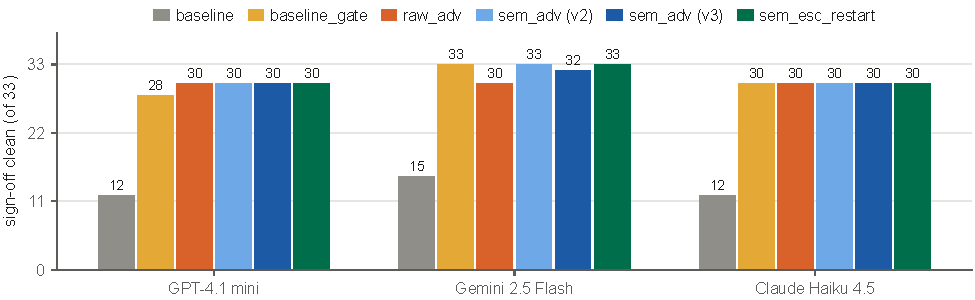
\includegraphics{fig_s_p3_api}
\caption{The three API ladder rows: sign-off clean of $33$ by condition.
Simulation alone signs off every sim-silent defect; any tool feedback repairs
them.}
\label{fig:s-p3-api}
\end{figure}

Every non-baseline miss of the three API models is on \texttt{Address\_select},
apart from two alarm-only runs on \texttt{riscv\_alu\_flags} for GPT-4.1 mini;
Gemini~2.5 Flash's misses are raw text ($3$ of $3$) and v3 ($1$ of $3$). In the
seven-model sensitivity pool (six models plus qwen2.5-coder:32b) every contrast
keeps its sign: escalation minus the alarm $+17.7$ (CI $+10.4$ to $+25.6$), v3
minus the alarm $+13.4$ (CI $+3.5$ to $+23.8$).

\subsection{Next steps from the case study}

Held-out defects for the v3 rules; a specification-valued default in the latch
directive; returning the best candidate so far (some runs pass simulation at some
point and lose it: $23$ of $198$ under v3 and $11$ under escalation in the $990$
runs); more replicates on the flat tasks (\texttt{noc\_xbar4},
\texttt{riscv\_alu\_flags}); and integration-level feedback.

% ============================================================================
\section{Statistics and Reproducibility}
\label{s:stats}

Rates carry Wilson $95\%$ intervals. Paired contrasts match runs on (model, task
or module, replicate); runs are independent draws, so the matching is a
stratification. Because the replicates of a cell are correlated, general claims
use the mean over cells of the within-cell rate difference, with a cell bootstrap
($10{,}000$ resamples, percentile interval) and a two-sided sign-flip
permutation test over cells ($20{,}000$ random sign patterns,
$p = (1 + \#\{|\bar d^{*}| \geq |\bar d|\}) / 20{,}001$), both seeded per label
(seed $20260925$ and the CRC of the label), so reruns reproduce byte for byte.
The Set~4 copy of these functions reproduces all twelve published Set~1 and
Set~3 values exactly before any contrast is reported. Per-model and per-task
Phase~3 breakdowns use run-level McNemar tests with Holm correction within each
contrast. The deficit figure uses Newcombe intervals for a difference of two
independent proportions.

Every table and figure can be regenerated from the repository; the commands and
the canonical evidence file for each section are listed in \texttt{REPO\_INDEX.md}.

\end{document}
